\subsection{Ensemble Toolkit}

An ensemble-based application is a \textbf{workflow}, i.e., a set of tasks
with dependencies that determine the order of their execution. Subsets of
these tasks can be \textbf{workloads}, i.e., tasks whose dependencies have
been satisfied at a particular time and may be executed concurrently.
Ensemble-based application vary in the type of coupling between tasks, the
frequency and volume of information exchanged between these tasks, and the
executable of each task. This type of applications requires specific
coordination, orchestration and execution protocols, posing both
domain-specific and engineering challenges.

Ensemble Toolkit (EnTK), the topmost layer of RCT, simplifies the process of
creating and executing ensemble-based applications with complex coordination
and communication requirements. EnTK decouples the description of
ensemble-based applications from their execution by separating three orders
of concern: specification of task and resource requirements; resource
selection and acquisition; and task execution management. Domain scientists
retain full control of the implementation of their algorithms by programming
ensemble-based applications by describing what should be executed, when it
should be executed and where it should be executed. EnTK automates the
process of acquiring the resources needed by those applications and managing
the task execution via a runtime system like RADICAL-Pilot.

% A key objective of EnTK is to provide a solution to the execution of
% ensemble-based applications that is independent of the nature of tasks.

EnTK has been previously used to develop the
ExTASY~\cite{balasubramanian2016extasy} framework for the execution of
MD-based advanced sampling methods. EnTK is also being utilized to develop
ensemble-based applications to execute workflows in the seismology and
climate science domains. Each application requires different workflows, with
different types of tasks, executed on specific HPC resources. EnTK supported
the development of a simulation-analysis execution pattern for ExTASY,
implementing two sampling algorithms for execution of both multithreaded and
MPI tasks on ARCHER, Stampede and Blue Waters HPC machines.

% EnTK is being
% used to develop inversion of full-waveform, wide-bandwidth data for seismic
% tomography, and a new downscaling methodology to quantify the photovoltaic
% (PV) energy potential in selected regions of the USA\@.

Currently, EnTK enables the execution of up to \(O(10^4)\) tasks on thousands
of CPU and GPU nodes on the resources of XSEDE, ORNL, NCSA, NWSC and UK NSS,
comprising a total of eight HPC machines. At this scale, multiple sources of failure
affect execution, producing loss of information and compute time. Thus, fault
tolerance and recovery capabilities are first order concerns of the design of
EnTK\@. As such, EnTK can handle task execution failures, resource-level
failures, and failures of its own subcomponents and subprocesses, including
network connectivity issues.

EnTK exposes to the end-user three components, namely \textbf{Pipeline},
\textbf{Stage} and \textbf{Task}, to create ensemble-based applications. Users
also use the \textbf{Application Manager} component to specify resources for
the execution of their ensemble-based application. Two internal components
called \textbf{WF Processor} and \textbf{Execution Manager} are used
to coordinate and enact the execution of the application (see
Figure~\ref{fig:entk_arch}).

\begin{figure}
  \centering
  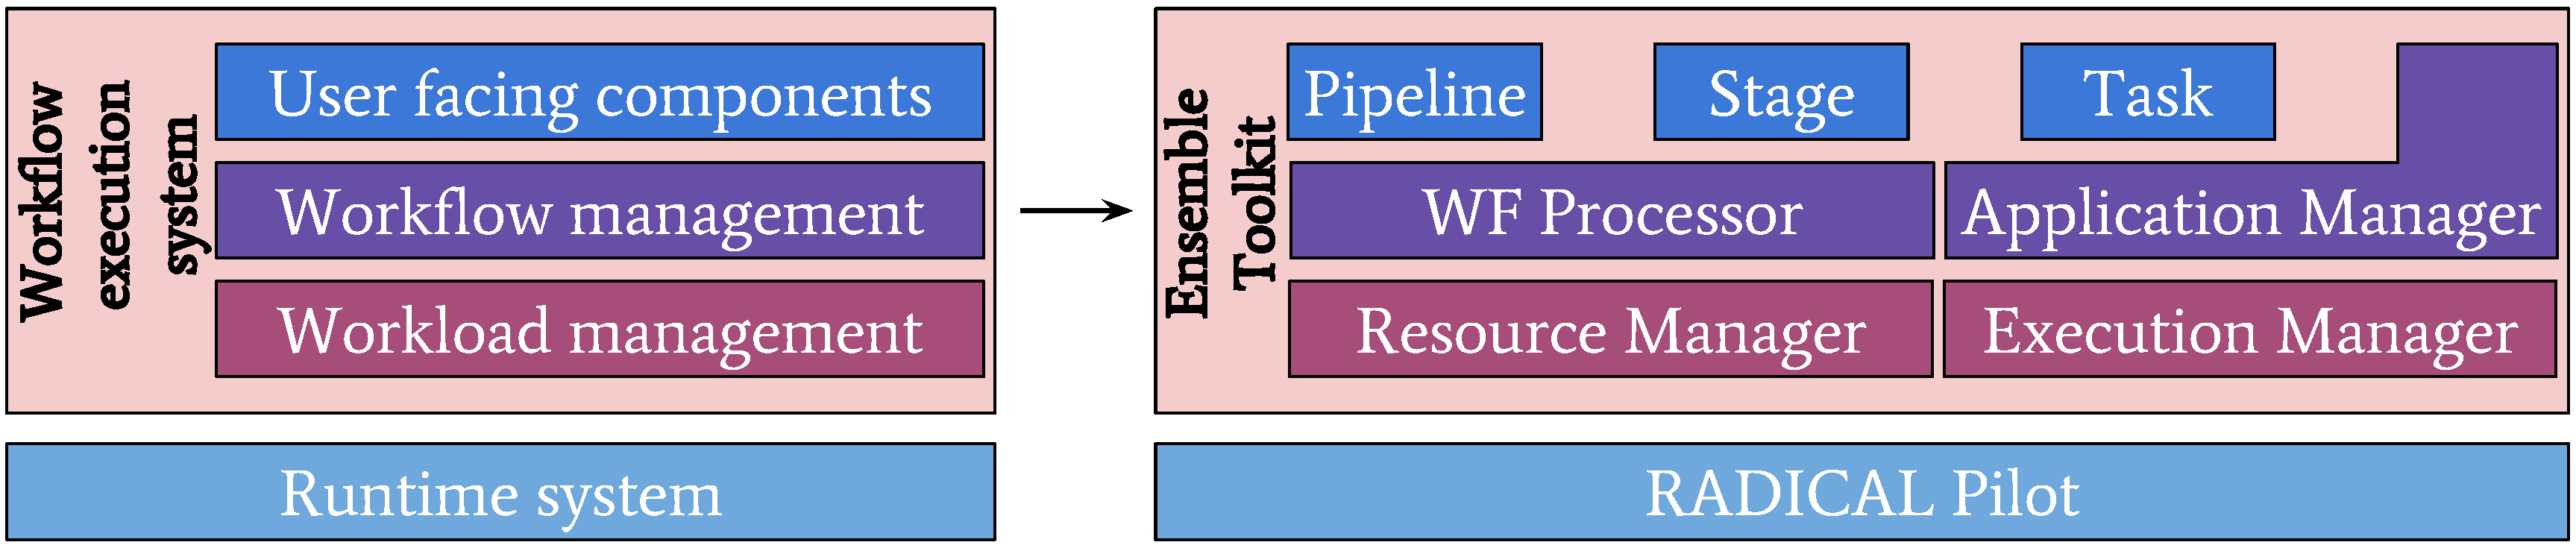
\includegraphics[width=\columnwidth]{FIGURES/entk_overview.pdf}
  \caption{\textbf{Left:} Ensemble Toolkit overview, showing how the abstract
           workflow execution system is mapped to specific components exposed
           to the users and components internal to the
           toolkit.}\label{fig:entk_arch}
\end{figure}

The Task component is used to encapsulate an executable  and its input/output
data, resource and software environment requirements. The Stage component is
used to group tasks that have the same dependencies and can be executed
concurrently. The Pipeline component is used to describe a sequence of
stages, i.e., operations that need to be executed sequentially, not concurrently.

EnTK enables users to program ensemble-based applications directly in Python,
without requiring knowledge of a domain-specific language. The use of the
Task, Stage, and Pipeline components, which are based on the well known set
and list data structures, avoids the need to express explicitly relationship
among tasks. These relationships are insured by design, depending on the
partitioning of the set of tasks into stages and then pipelines. Further,
EnTK enables an explicit definition of pre and post conditions on the
execution of tasks, stages, and pipelines, enabling a fine grained
adaptivity, both a local and global level. Conveniently, this does not
require the codification of a directed acyclic graph (DAG), a process that imposes a rigid
representation model on the domain scientists.

% The \textbf{Application Manager} component of EnTK enables users to specify
% target resources for the execution of the ensemble-based application. This
% includes properties like walltime, number of nodes and credentials for
% resource access. Users can also define execution setup parameters such as
% the number of processes or messaging queues that should be used by EnTK\@.
% This allow to size and tune the performance of EnTK, depending on the
% number of tasks, stages and pipelines, but also on the resources available
% to the toolkit.

% The Application Manager along with the \textbf{WF Processor} is responsible
% for the transformation of the application workflow into a sequence of tasks
% that can be submitted to the indicated resources for execution. Internally,
% the \textbf{Resource Manager} and \textbf{Execution Manager} components
% enable the acquisition of resources and the management of execution of
% these workloads (see \textbf{Figure~\ref{fig:entk_arch}}, right schematic
% of left panel).

Once the workflow of an ensemble-based application is described, one or more
pipelines are submitted to the Application Manager module for execution. The
Application Manager sets up multiple processes, threads and a messaging
infrastructure for communication. The WF Processor processes each pipeline,
identifying tasks which have their dependencies satisfied and can be executed
concurrently. These tasks are handed over to the Execution Manager that binds
tasks to resources on the basis of a set of heuristics called ``execution
strategies''. The Execution Manager uses the underlying runtime system,
RADICAL-Pilot, to execute the tasks on the specific target resource.

EnTK is implemented as a multiprocess application. The number of processes
can be tuned to match the throughput requirements of ensemble-based
applications and the capabilities of diverse target resources. All but the
master process of the toolkit are stateless, enabling process-level fault
tolerance. Upon failure of one or more stateless processes, application tasks
can be assigned to existing or newly created processes without blocking the
overall execution. Upon failure of the master process, execution can be
restarted without loosing data about tasks that have been already executed.

% A description of the set of resources to be utilized is provided to the
% \textbf{Application Manager}.
